% GNUPLOT: LaTeX picture with Postscript
\begingroup
  \makeatletter
  \providecommand\color[2][]{%
    \GenericError{(gnuplot) \space\space\space\@spaces}{%
      Package color not loaded in conjunction with
      terminal option `colourtext'%
    }{See the gnuplot documentation for explanation.%
    }{Either use 'blacktext' in gnuplot or load the package
      color.sty in LaTeX.}%
    \renewcommand\color[2][]{}%
  }%
  \providecommand\includegraphics[2][]{%
    \GenericError{(gnuplot) \space\space\space\@spaces}{%
      Package graphicx or graphics not loaded%
    }{See the gnuplot documentation for explanation.%
    }{The gnuplot epslatex terminal needs graphicx.sty or graphics.sty.}%
    \renewcommand\includegraphics[2][]{}%
  }%
  \providecommand\rotatebox[2]{#2}%
  \@ifundefined{ifGPcolor}{%
    \newif\ifGPcolor
    \GPcolorfalse
  }{}%
  \@ifundefined{ifGPblacktext}{%
    \newif\ifGPblacktext
    \GPblacktexttrue
  }{}%
  % define a \g@addto@macro without @ in the name:
  \let\gplgaddtomacro\g@addto@macro
  % define empty templates for all commands taking text:
  \gdef\gplbacktext{}%
  \gdef\gplfronttext{}%
  \makeatother
  \ifGPblacktext
    % no textcolor at all
    \def\colorrgb#1{}%
    \def\colorgray#1{}%
  \else
    % gray or color?
    \ifGPcolor
      \def\colorrgb#1{\color[rgb]{#1}}%
      \def\colorgray#1{\color[gray]{#1}}%
      \expandafter\def\csname LTw\endcsname{\color{white}}%
      \expandafter\def\csname LTb\endcsname{\color{black}}%
      \expandafter\def\csname LTa\endcsname{\color{black}}%
      \expandafter\def\csname LT0\endcsname{\color[rgb]{1,0,0}}%
      \expandafter\def\csname LT1\endcsname{\color[rgb]{0,1,0}}%
      \expandafter\def\csname LT2\endcsname{\color[rgb]{0,0,1}}%
      \expandafter\def\csname LT3\endcsname{\color[rgb]{1,0,1}}%
      \expandafter\def\csname LT4\endcsname{\color[rgb]{0,1,1}}%
      \expandafter\def\csname LT5\endcsname{\color[rgb]{1,1,0}}%
      \expandafter\def\csname LT6\endcsname{\color[rgb]{0,0,0}}%
      \expandafter\def\csname LT7\endcsname{\color[rgb]{1,0.3,0}}%
      \expandafter\def\csname LT8\endcsname{\color[rgb]{0.5,0.5,0.5}}%
    \else
      % gray
      \def\colorrgb#1{\color{black}}%
      \def\colorgray#1{\color[gray]{#1}}%
      \expandafter\def\csname LTw\endcsname{\color{white}}%
      \expandafter\def\csname LTb\endcsname{\color{black}}%
      \expandafter\def\csname LTa\endcsname{\color{black}}%
      \expandafter\def\csname LT0\endcsname{\color{black}}%
      \expandafter\def\csname LT1\endcsname{\color{black}}%
      \expandafter\def\csname LT2\endcsname{\color{black}}%
      \expandafter\def\csname LT3\endcsname{\color{black}}%
      \expandafter\def\csname LT4\endcsname{\color{black}}%
      \expandafter\def\csname LT5\endcsname{\color{black}}%
      \expandafter\def\csname LT6\endcsname{\color{black}}%
      \expandafter\def\csname LT7\endcsname{\color{black}}%
      \expandafter\def\csname LT8\endcsname{\color{black}}%
    \fi
  \fi
  \setlength{\unitlength}{0.0500bp}%
  \begin{picture}(7000.00,3500.00)%
    \gplgaddtomacro\gplbacktext{%
    \put(0,0){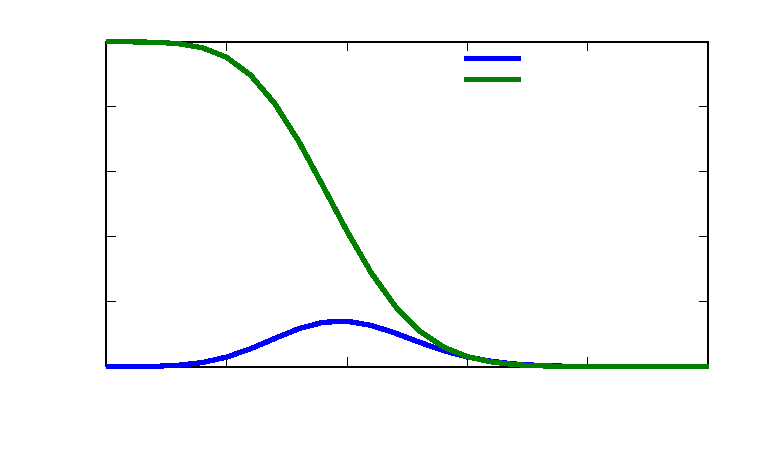
\includegraphics{OC-Funktion2}}
    \thicklines
      \colorrgb{0.00,0.00,0.00}%
      \put(740,640){\makebox(0,0)[r]{\strut{}0}}%
      \colorrgb{0.00,0.00,0.00}%
      \put(740,1264){\makebox(0,0)[r]{\strut{}0.2}}%
      \colorrgb{0.00,0.00,0.00}%
      \put(740,1888){\makebox(0,0)[r]{\strut{}0.4}}%
      \colorrgb{0.00,0.00,0.00}%
      \put(740,2511){\makebox(0,0)[r]{\strut{}0.6}}%
      \colorrgb{0.00,0.00,0.00}%
      \put(740,3135){\makebox(0,0)[r]{\strut{}0.8}}%
      \colorrgb{0.00,0.00,0.00}%
      %%%%%%%%%%
      
      
      \put(860,3759){\makebox(0,0)[r]{\strut{}1}}%
      \colorrgb{0.00,0.00,0.00}%
      \put(860,440){\makebox(0,0){\strut{}0}}%
      \colorrgb{0.00,0.00,0.00}%
      \put(2016,440){\makebox(0,0){\strut{}0.1}}%
      \colorrgb{0.00,0.00,0.00}%
      \put(3172,440){\makebox(0,0){\strut{}0.2}}%
      \colorrgb{0.00,0.00,0.00}%
      \put(4327,440){\makebox(0,0){\strut{}0.3}}%
      \colorrgb{0.00,0.00,0.00}%
      \put(5483,440){\makebox(0,0){\strut{}0.4}}%
      \colorrgb{0.00,0.00,0.00}%
      \put(6639,440){\makebox(0,0){\strut{}0.5}}%
      \colorrgb{0.00,0.00,0.00}%
      \put(160,2199){\rotatebox{90}{\makebox(0,0){\strut{}$L, p_i$}}}%
      \colorrgb{0.00,0.00,0.00}%
      \put(6000,440){\makebox(0,0){\strut{}$p$}}%
    }%
    \gplgaddtomacro\gplfronttext{%
      \colorrgb{0.00,0.00,0.00}%
      \put(6519,3596){\makebox(0,0)[r]{\strut{}$p_i(N, M, n)$}}%
      \colorrgb{0.00,0.00,0.00}%
      \put(6519,3396){\makebox(0,0)[r]{\strut{}$L(p, M, N, c)$}}%
    }%
    \gplbacktext
    %\put(0,0){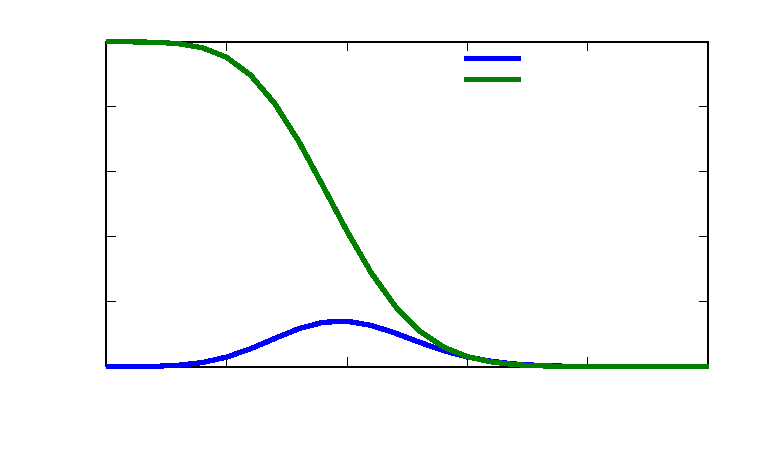
\includegraphics{OC-Funktion2}}%
    \gplfronttext \pause
    \put(2030,3600){\color{red!80!black}
      \put(0,0){\line(-1,0){1180}}
      \put(0,0){\line(0,-1){2960}}
      \put(0,0){\circle*{80}}
      \put(50,0){\makebox(0,0)[l]{\strut{}Produzentenpunkt}}
      \put(-1220,0){\makebox(0,0)[r]{\strut{}$1-\alpha$}}
      \put(0,-3400 ){\makebox(0,0)[c]{\strut{}AQL}}} \pause
      %%%
      \put(3020,2200){\color{red!80!black}
      \put(0,0){\line(-1,0){2160}}
      \put(0,0){\line(0,-1){1550}}
      \put(0,0){\circle*{80}}
      %\put(50,0){\makebox(0,0)[l]{\strut{}Produzentenpunkt}}
      \put(-2200,0){\makebox(0,0)[r]{\strut{}$0{,}5$}}
      \put(0,-2000 ){\makebox(0,0)[c]{\strut{}IQL}}} \pause
      %%%
      \put(3850,1000){\color{red!80!black}
      \put(0,0){\line(-1,0){3000}}
      \put(0,0){\line(0,-1){350}}
      \put(0,0){\circle*{80}}
      \put(50,0){\makebox(0,0)[l]{\strut{}Konsumentenpunkt}}
      \put(-3040,0){\makebox(0,0)[r]{\strut{}$\beta$}}
      \put(0,-800 ){\makebox(0,0)[c]{\strut{}RQL}}}
  \end{picture}%
\endgroup
